\documentclass[oneside,openany,headings=optiontotoc,11pt,numbers=noenddot]{article}

\usepackage[a4paper]{geometry}
\usepackage[utf8]{inputenc}
\usepackage[T1]{fontenc}
\usepackage{lmodern}
\usepackage[ngerman]{babel}
\usepackage{ngerman}

\usepackage[onehalfspacing]{setspace}

\usepackage{fancyhdr}
\usepackage{fancybox}

\usepackage{rotating}
\usepackage{varwidth}

%Struktogramme
\usepackage[german,curves]{struktex}

\usepackage{pdflscape}
\usepackage{changepage}
\usepackage{graphicx}
\usepackage[bottom]{footmisc}
\usepackage{transparent}
\usepackage{graphbox}
\graphicspath{
	{Pics/PDFs/}
	{Pics/JPGs/}
	{Pics/PNGs/}
}
\usepackage{caption}
\usepackage{wrapfig}
\usepackage{marginnote}
\usepackage{tabularx}
\usepackage{dashrule}
\usepackage{soulutf8}
\usepackage{hhline}
%arydshln suppresses vertical lines in table
%\usepackage{arydshln}
\usepackage{multirow}
\usepackage{enumerate}
\usepackage[hidelinks]{hyperref}
\usepackage{listings}

\usepackage[table]{xcolor}
\usepackage{array}
\usepackage{enumitem,amssymb,amsmath}
\usepackage{interval}
\usepackage{cancel}
\usepackage{stmaryrd}
\usepackage{wasysym}
\usepackage{polynom}
\usepackage{diagbox}
\usepackage{dashrule}
\usepackage{framed}
\usepackage{mdframed}
\usepackage{karnaugh-map}
\usepackage{pdfpages}

\usepackage{blindtext}

\usepackage{eso-pic}

\usepackage{amssymb}
\usepackage{eurosym}

\usepackage[pages=some]{background}
\pagestyle{headings}
\renewcommand{\headrulewidth}{0.2pt}
\renewcommand{\footrulewidth}{0.2pt}
\newcommand*{\underdownarrow}[2]{\ensuremath{\underset{\overset{\Big\downarrow}{#2}}{#1}}}
\setlength{\fboxsep}{5pt}
\newcommand{\explainBelow}[3]{\underbrace{#1}_{\parbox{\widthof{#3}}{\footnotesize\raggedright #2}}}
\newcommand{\explainAbove}[3]{\overbrace{#1}^{\parbox{\widthof{#3}}{\footnotesize\raggedright #2}}}
\newcommand\footnoteref[1]{\protected@xdef\@thefnmark{\ref{#1}}\@footnotemark}


% Codestyle defined
\definecolor{codegreen}{rgb}{0,0.6,0}
\definecolor{codegray}{rgb}{0.5,0.5,0.5}
\definecolor{codepurple}{rgb}{0.58,0,0.82}
\definecolor{backcolour}{rgb}{0.95,0.95,0.92}
\definecolor{deepgreen}{rgb}{0,0.5,0}
\definecolor{darkblue}{rgb}{0,0,0.65}
\definecolor{mauve}{rgb}{0.40, 0.19,0.28}
\colorlet{exceptioncolour}{yellow!50!red}
\colorlet{commandcolour}{blue!60!black}
\colorlet{numpycolour}{blue!60!green}
\colorlet{specmethodcolour}{violet}

%Neue Spaltendefinition
\newcolumntype{L}[1]{>{\raggedright\let\newline\\\arraybackslash\hspace{0pt}}m{#1}}
\newcolumntype{M}{>{\centering\arraybackslash}X}
\newcommand{\cmnt}[1]{\ignorespaces}
%Textausrichtung ändern
\newcommand\tabrotate[1]{\rotatebox{90}{\raggedright#1\hspace{\tabcolsep}}}

%Intervall-Konfig
\intervalconfig {
	soft open fences
}

%Bash
\lstdefinestyle{BashInputStyle}{
	language=bash,
	basicstyle=\small\sffamily,
	backgroundcolor=\color{backcolour},
	columns=fullflexible,
	backgroundcolor=\color{backcolour},
	breaklines=true,
}
%Java
\lstdefinestyle{JavaInputStyle}{
	language=Java,
	backgroundcolor=\color{backcolour},
	aboveskip=1mm,
	belowskip=1mm,
	showstringspaces=false,
	columns=flexible,
	basicstyle={\footnotesize\ttfamily},
	numberstyle={\tiny},
	numbers=none,
	keywordstyle=\color{purple},,
	commentstyle=\color{deepgreen},
	stringstyle=\color{blue},
	emph={out},
	emphstyle=\color{darkblue},
	emph={[2]rand},
	emphstyle=[2]\color{specmethodcolour},
	breaklines=true,
	breakatwhitespace=true,
	tabsize=2,
}
%Python
\lstdefinestyle{PythonInputStyle}{
	language=Python,
	alsoletter={1234567890},
	aboveskip=1ex,
	basicstyle=\footnotesize,
	breaklines=true,
	breakatwhitespace= true,
	backgroundcolor=\color{backcolour},
	commentstyle=\color{red},
	otherkeywords={\ , \}, \{, \&,\|},
	emph={and,break,class,continue,def,yield,del,elif,else,%
		except,exec,finally,for,from,global,if,import,in,%
		lambda,not,or,pass,print,raise,return,try,while,assert},
	emphstyle=\color{exceptioncolour},
	emph={[2]True,False,None,min},
	emphstyle=[2]\color{specmethodcolour},
	emph={[3]object,type,isinstance,copy,deepcopy,zip,enumerate,reversed,list,len,dict,tuple,xrange,append,execfile,real,imag,reduce,str,repr},
	emphstyle=[3]\color{commandcolour},
	emph={[4]ode, fsolve, sqrt, exp, sin, cos, arccos, pi,  array, norm, solve, dot, arange, , isscalar, max, sum, flatten, shape, reshape, find, any, all, abs, plot, linspace, legend, quad, polyval,polyfit, hstack, concatenate,vstack,column_stack,empty,zeros,ones,rand,vander,grid,pcolor,eig,eigs,eigvals,svd,qr,tan,det,logspace,roll,mean,cumsum,cumprod,diff,vectorize,lstsq,cla,eye,xlabel,ylabel,squeeze},
	emphstyle=[4]\color{numpycolour},
	emph={[5]__init__,__add__,__mul__,__div__,__sub__,__call__,__getitem__,__setitem__,__eq__,__ne__,__nonzero__,__rmul__,__radd__,__repr__,__str__,__get__,__truediv__,__pow__,__name__,__future__,__all__},
	emphstyle=[5]\color{specmethodcolour},
	emph={[6]assert,range,yield},
	emphstyle=[6]\color{specmethodcolour}\bfseries,
	emph={[7]Exception,NameError,IndexError,SyntaxError,TypeError,ValueError,OverflowError,ZeroDivisionError,KeyboardInterrupt},
	emphstyle=[7]\color{specmethodcolour}\bfseries,
	emph={[8]taster,send,sendMail,capture,check,noMsg,go,move,switch,humTem,ventilate,buzz},
	emphstyle=[8]\color{blue},
	keywordstyle=\color{blue}\bfseries,
	rulecolor=\color{black!40},
	showstringspaces=false,
	stringstyle=\color{deepgreen}
}

\lstset{literate=%
	{Ö}{{\"O}}1
	{Ä}{{\"A}}1
	{Ü}{{\"U}}1
	{ß}{{\ss}}1
	{ü}{{\"u}}1
	{ä}{{\"a}}1
	{ö}{{\"o}}1
}

% Neue Klassenarbeits-Umgebung
\newenvironment{worksheet}[3]
% Begin-Bereich
{
	\newpage
	\sffamily
	\setcounter{page}{1}
	\ClearShipoutPicture
	\AddToShipoutPicture{
		\put(55,761){{
				\mbox{\parbox{385\unitlength}{\tiny \color{codegray}BBS I Mainz, #1 \newline #2
						\newline #3
					}
				}
			}
		}
		\put(455,761){{
				\mbox{\hspace{0.3cm}
\includegraphics[width=0.2\textwidth]{../../logo.pdf}}
			}
		}
	}
}
% End-Bereich
{
	\clearpage
	\ClearShipoutPicture
}

\pagestyle{plain}

\geometry{left=1.50cm,right=1.50cm,top=2.50cm,bottom=1.00cm,includeheadfoot}

\begin{document}
	\begin{worksheet}{BS EGSIE 18}{1. Lehrjahr, LF 4 - Informationstechnische Systeme bereitstellen}{Verarbeitungsgeräte - Intern}
		\onehalfspacing
		\clearpage
		\setcounter{page}{3}
		\setcounter{section}{1}
		\setcounter{subsection}{1}
		\subsection{Datenverarbeitung im PC}
		\subsubsection*{Interne Komponenten}
		\begin{framed}
			\renewcommand{\arraystretch}{1.25}
			\begin{tabularx}{\textwidth}{cMcM}
				Netzteil & Massenspeicher & Arbeitsspeicher & CPU (Central Processing Unit)\\
				Chipsatz & Motherboard & Cores & CPU\\
				Controller & Mainboard & Bussysteme
			\end{tabularx}
		\end{framed}
		Ein Computer besitzt als Verarbeitungsgeräte verschiedene Komponenten. Diese übernehmen dabei folgende Aufgaben:
		\begin{itemize}
			\item mindestens eine \underline{\color{white}{CPU (Central Processing Unit)CPU (Central Processing Unit)}} zur eigentlichen Datenverarbeitung.\\
			Diese besteht häufig aus verschiedenen \underline{\color{white}{CPUCPUCPU}}-Kernen, auch als \underline{\color{white}{CoresCoresCores}} bezeichnet. Diese Cores können getrennte Rechenaufgaben durchführen.
			\item \underline{\color{white}{ArbeitsspeicherArbeitsspeicherArbeitsspeicher}} zur vorübergehenden Ablage von Informationen
			\item sowie verschiedene Schnittstellen und Peripheriegeräte, die den Informationsaustausch mit der Umgebung übernehmen
			\begin{itemize}
				\item \underline{\color{white}{ChipsatzChipsatzChipsatz}} und \underline{\color{white}{ControllerControllerController}}
				\item \underline{\color{white}{BussystemeBussystemeBussysteme}}
				\item \underline{\color{white}{MassenspeicherMassenspeicherMassenspeicher}} zur dauerhaften Ablage von Informationen und Programmen
			\end{itemize}
		\end{itemize}
		Abgesehen vom Massenspeicher werden die übrigen Komponenten üblicherweise zusammen auf einer gemeinsamen Leiterplatte verbaut. Diese Leiterplatte bezeichnet man als \underline{\color{white}{MainboardMainboardMainboard}} oder auch \underline{\color{white}{MotherboardMotherboardMotherboard}}. Die Energieversorgung der verbauten Komponenten übernimmt das sogenannte \underline{\color{white}{NetzteilNetzteilNetzteil}}.\\
		\par\noindent
		Ein weit verbreitetes Konzept für den Aufbau dieser Verarbeitungsgeräte ist die \textbf{Von-Neumann-Architektur}. Sie bündelt im wesentlichen vier Funktionseinheiten:\\
		\par\noindent
		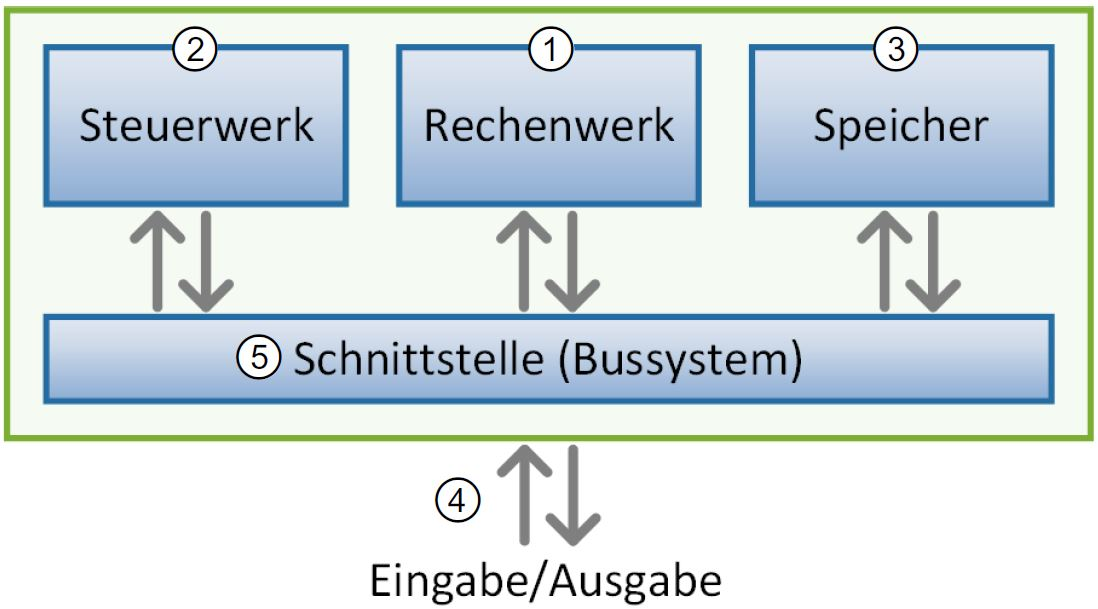
\includegraphics[width=\textwidth]{../99_Bilder/VNA.jpg}\\
		\par\noindent
		Das \textbf{Bussystem} dient als Kommunikationsbrücke der Komponenten mit der Außenwelt.
		\subsubsection*{Die Bestandteile des Mainboard}
		Auf dieser Leiterplatte werden die meisten Kernkomponenten des Verarbeitungsgeräts zusammengefasst.\\
		\par\noindent
		\begin{minipage}{0.35\textwidth}
			\begin{enumerate}
				\item Prozessor mit Kühlkörper und Lüfter
				\item Steckplätze für den Arbeitsspeicher
				\item 24-poliger Anschluss für die Stromversorgung
				\item achtpoliger EPS12V-Anschluss für zusätzliche Stromversorgung
				\item ATX-Anschlussfeld mit externen Anschlüssen
				\item Heatpipe-Kühlung für Chipsatz und Spannungsregler
				
			\end{enumerate}
		\end{minipage}
		\hfill
		\begin{minipage}{0.6\textwidth}
			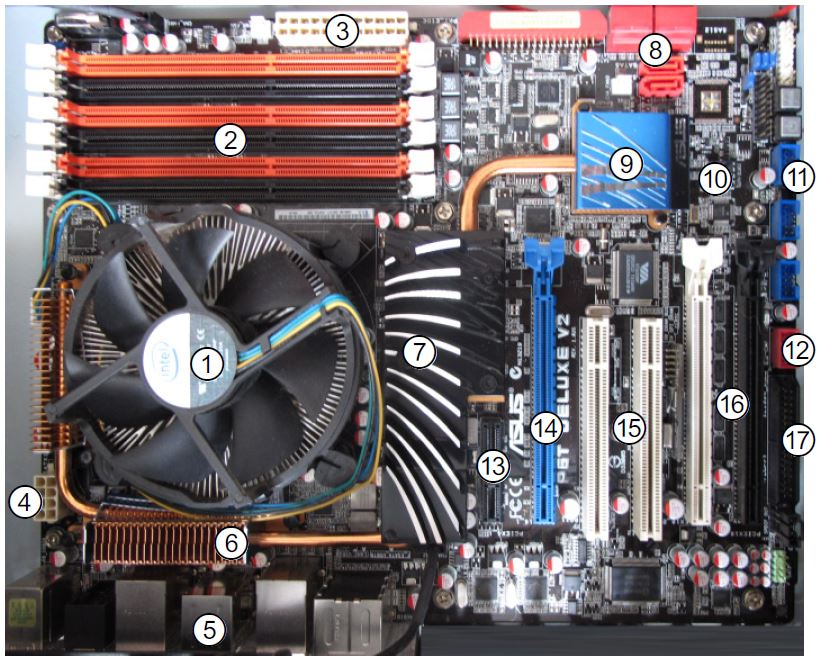
\includegraphics[width=0.95\textwidth]{../99_Bilder/MB.jpg}
		\end{minipage}
		\vfill
		\begin{enumerate}
			\setcounter{enumi}{6}
			\item Kühlkörper über den Spannungsreglern
			\item SATA-Anschlüsse für interne Laufwerke
			\item Chipsatz
			\item BIOS-Chip
			\item Anschlüsse für externe USB
			\item Anschlüsse für FireWire
			\item Steckplatz für PCI-Express (PCIe) x4
			\item Grafikkarten-Steckplatz PEG (PCIe x16)
			\item PCI-Steckplätze (32 Bit, 66MHz)
			\item Steckplätze PCI Express (PCIe) x16
			\item IDE/PATA-Anschluss
		\end{enumerate}
		\subsubsection*{Pin-Sockel für den Prozessor}
		Um die Prozessoren auf dem Mainboard zu befestigen, stehen diverse Sockel-Arten zur Verfügung.\\
		Der ZIF-Sockel (Zero Insertion Force) ermöglicht das Einsetzen des Prozessors ohne zusätzlichen Krafteinwirkung.\\
		\footnotesize{Zu beachten ist, dass sowohl Intel wie auch AMD verschiedene Sockel mit einer unterschiedlichen Anzahl und Anordnung von Pins entwickelt.}\normalsize\\
		Die derzeit verbreiteten Sockel ermöglichen die Nutzung unterschiedlicher Prozessoren mit verschiedenen Taktfrequenzen. Diese Taktfrequenz berechnet sich aus dem internen Multiplikator und der Taktfrequenz des Chipsatzes (auch Front Size Bus (FSB) genannt).\\
		Bei aktuellen Prozessoren sind die Speichercontroller per Hyper-Transport-Verbindung an die Northbridge angebunden und somit auf dem Prozessor integriert. In solchen Fällen lässt sich die Taktfrequenz aus dem Referenztakt von 200 MHz multipliziert mit dem entsprechenden CPU-Multiplikator.
		\par\noindent
		Aufgrund verschiedener Protokolle der Datenübertragung zwischen Prozessor und Hauptspeicher kann der Zugriff beschleunigt werden.
		\subsection*{Mainboard-Formfaktor}
		Bei den einzelnen Mainboards gibt es Unterschiede bei den Abmessungen, auch \textbf{Formfaktor} genannt.\\
		Aus dem Formfaktor lässt sich zusätzlich zur Abmessung auch die Art und Lage der Bauteile und der Schnittstelle bestimmen.\\
		\par\noindent
		\begin{tabularx}{\textwidth}{|X|X|X|}
			\hline
			\rowcolor{gray!15} \textit{Formfaktor} & \textit{Abmessung (Breite x Länge)} & \textit{Beschreibung}\\
			\hline
			\hline
			\textit{Extended ATX (EATX)} & 305 mm x 330 mm & 2 Prozessorsockel, Server-Board für Racks\\
			\hline
			\textit{ATX} & 305 mm x 244 mm & sehr weit verbreitet\\
			\hline
			\textit{microATX ( $\mu$ATX)} & 244 mm x 244 mm &  ebenfalls sehr gebräuchlich\\
			\hline
			\textit{Flex-ATX} & 229 mm x 191 mm & Thin-Clients und HTPCs (Intel Atom, Via Nano)\\
			\hline
		\end{tabularx}
		\begin{tabularx}{\textwidth}{|X|X|X|}
			\hline
			\rowcolor{gray!15} \textit{Formfaktor} & \textit{Abmessung (Breite x Länge)} & \textit{Beschreibung}\\
			\hline
			\hline
			\textit{Mini-ITX} & 170 mm x 170 mm & Thin-Clients und HTPCs\\
			\hline
			\textit{Nano-ITX} & 120 mm x 120 mm & Thin-Clients und HTPCs\\
			\hline
			\textit{BTX} & 325 mm x 267 mm & konnte sich als ATX-Nachfolger nicht durchsetzen\\
			\hline
			\textit{microBTS ($\mu$BT)} & 264 mm x 267 mm & ebenfalls selten zu finden\\
			\hline
		\end{tabularx}\\
		\par\noindent
		Durch den Formfaktor wird außerdem der Gehäusetyp und das verwendbare Netzteil bestimmt.\\
		Grundsätzlich passen ATX- bzw. microATX-Mainboards \underline{nicht} in BTX- oder ITX-Gehäuse.
	\end{worksheet}
\end{document}